%!TEX root = info-main.tex
% ** Section 2 **

\section{System Model and Problem Formulation}

In this section, we present the network, channel and capture models,
and describe selfish misbehavior in Wi-Fi tethering.

\subsection{Network Model}
%
\begin{figure}[hbt]
 \center{
        \scalebox{0.4}{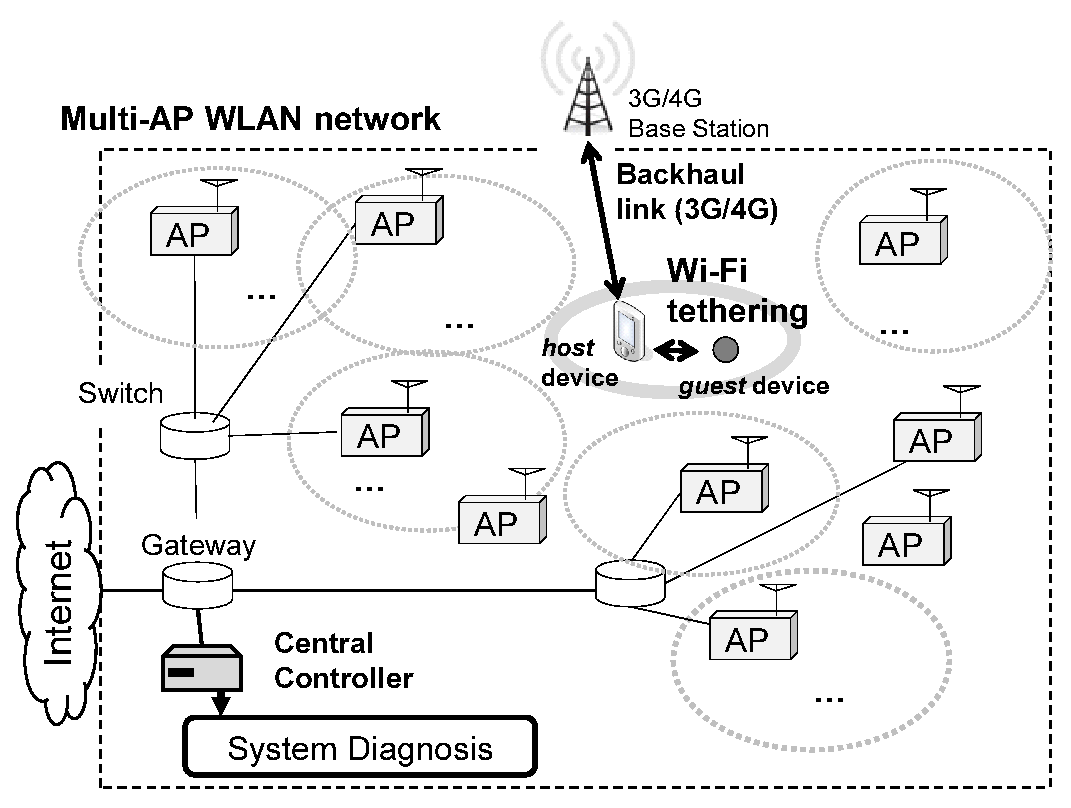
\includegraphics{./figures/FIG_architecure.eps}}
 \caption{Illustration of the problem: selfish misconfigured Wi-Fi tethering
 sets up the network in a centrally managed multi-AP network}
 \label{fig-architecture}
 }
\end{figure}
%
We consider a scenario in which an unauthorized Wi-Fi tethering system
sets up a Wi-Fi hotspot within a centrally managed Wi-Fi network,
where the network consists of a central \emph{controller} and
$N$ 802.11 access points (APs), $A=\{AP_1, AP_2, \cdots, AP_N\}$,
as illustrated in Fig.~\ref{fig-architecture}.
%
%The launched tethering consists of an Internet-connected
The tethering consists of an Internet-connected
(e.g., through 3G/4G cellular connection) mobile phone and a
tethered Wi-Fi-enabled device, contending for channel access
with nearby Wi-Fi systems.
% alex: why do we introduce this metric B_cel here?
Let $B_{cel}$ denote the capacity of the cellular backhaul link.
%
We will henceforth refer to the mobile device and the tethered
Wi-Fi device as \emph{host} and \emph{guest} nodes, respectively;
the \emph{host} node shares its 3G/4G Internet connection
with the \emph{guest} nodes via its Wi-Fi interface.
%

We assume that the multi-AP network is monitored and managed by the
controller, as shown in Fig.~\ref{fig-architecture}. Each $AP_i$
($AP_i \in A$) monitors the channel access activity and reports the
information to the controller periodically.
%
We also assume that frequency planning for each AP in the network
has been done {\em a priori} through a proper channel allocation algorithm
(e.g., \cite{Mishra_MC2R_2005, client_driven06, Mishra_06}), % TODO:add ref
so as to minimize inter-AP inference on each AP.

\subsection{Channel Model}
%
For a given link, let $s$ and $r$ denote the transmitter node
and its corresponding receiver node of a link, respectively.
The distance between the two nodes $s$ and $r$ is
denoted by $d_{s,r}$.
%
We assume that the channel gain $G_{s,r}$ between the transmitter $s$
and the receiver $r$ is determined based on the log-distance
path-loss model described in~\cite{Tse:Viswanath05}:
\begin{equation} \label{eq:pathloss}
G_{s,r} = \frac{1}{{d_{s,r}}^{\alpha}},
\end{equation}
where $\alpha$ is the path-loss exponent (normally, ranging from 2 to 5).
%
Let $P_{s}$ and $P_{r}$ denote the transmission power of node $s$
and the received power at $r$, respectively.
We assume that all the transmitters transmit frames at the same
nominal power $P_{0}$.
%
Then, $P_{r}$ is expressed as $P_{r}=G_{s,r}P_{0}$.
%
The received signal to interference ratio (SIR) $SIR_{r}$
at the receiver is expressed as
\begin{equation}
SIR_{r} = \frac{G_{s,r}P_{0}}{\sum_{k\neq i}{G_{k, r}P_{0}}}.
\end{equation}

Let $\gamma_{m}$ denote the minimum SIR requirement (i.e., SIR threshold)
for successful reception at a receiver node under modulation
scheme $m$, where we consider multi-rate MAC as in 802.11a/b/g/n.

%% [TODO:] .. Error Probability..

%\subsection{802.11 MAC Protocol}

% alex-start
\subsection{Capture Model}
%\emph{Capture Model:}
% alex-end
%
Even when multiple independent transmissions occur simultaneously
to a receiver, the receiver can successfully capture the signal of
interest (SoI) if the received SIR is higher than a certain SIR
threshold, which is known as the {\em capture effect}~\cite{jlee:ychoi07}.

There are two well-known concurrent transmission technologies:
PHY capture effect~\cite{capture} and message-in-message (MIM)
\cite{jlee:ychoi07, MIM}.
Fig.~\ref{fig:capture} illustrates the main difference between PHY
capture and MIM.
%
%
\begin{figure} [t]
\center
  \subfigure[PHY capture effect]{
      \scalebox{0.45}{
      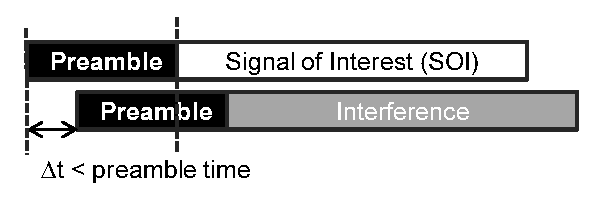
\includegraphics[trim=0.0cm 0.25cm 0.0cm 0.0cm]{./figures/FIG_capture_a_PHY}}
      }\\
  \subfigure[MIM (Message-In-Message)]{
      \scalebox{0.45}{
       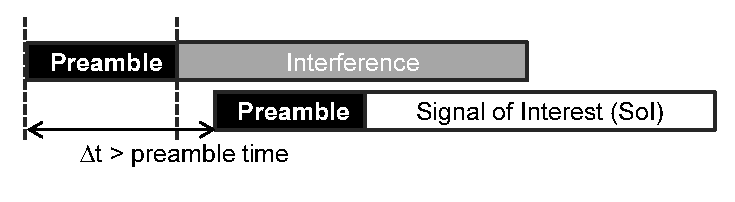
\includegraphics[trim=0.0cm 0.25cm 0.0cm 0.0cm]{./figures/FIG_capture_b_MIM}}
       }
  \subfigure[Adversary Model]{
      \scalebox{0.45}{ \label{fig:capture_c}
       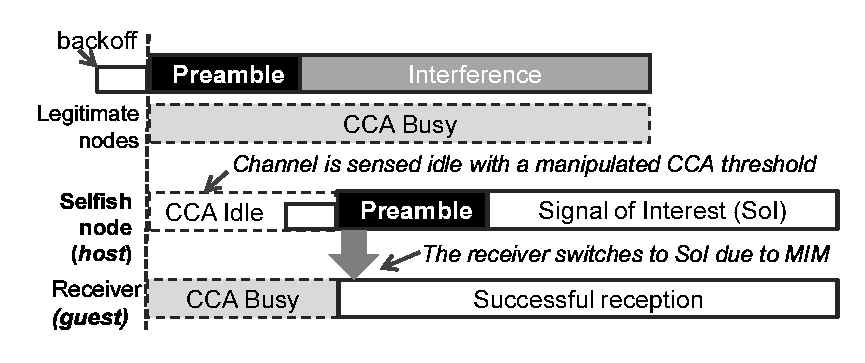
\includegraphics[trim=0.0cm 0.25cm 0.0cm 0.0cm]{./figures/FIG_capture_c_MIM}}
  }
  \caption{(a) PHY capture effect allows a receiver to successfully capture
    the signal of interest (SoI) if its Tx power is sufficiently higher
    than the sum of interferences. (b) MIM (Message-In-Message) allows
    a receiver to disengage from an ongoing packet reception, and
    engage in a new, stronger packet. (c) Selfish behavior with CCA manipulation exploits
    the benefits of MIM if the selfish pair (e.g., tethering link) has a short link distance.}
    \label{fig:capture}
\end{figure}
%
%
The PHY capture effect is the property of 802.11 radios, where
an SoI can be decoded successfully even when the interference arrives
at the same time, as long as the overlap \emph{within} the preamble
detection stage and the SoI is stronger than a specific threshold,
which we call the \emph{capture threshold}.
%
MIM is an enhanced PHY-layer capability that enables a receiver to
decode an SoI even if the SoI arrives after the preamble time of
the interference.
%
Specifically, MIM allows a receiver to disengage from the current
on-going frame reception and re-engage in a new, stronger frame.
However, MIM requires a higher SIR than the PHY capture, which we call
this SIR value the \emph{MIM threshold}, $\beta_{m}$, for modulation
scheme $m$.
%
These capture and MIM thresholds can vary~\cite{Ware:Dut00,
jlee:ychoi07}, particularly depending on the modulation
scheme~\cite{jlee:ychoi07}.

Throughput the paper, we assume that a receiver can decode a frame
successfully with probability greater than 0.9 when the received
SINR is consistently above the SIR threshold for a given modulation scheme.
%
We use the experimental results in~\cite{jlee:ychoi07} to configure
the SIR threshold $\gamma_{m}$ and MIM threshold $\beta_{m}$ for
modulation scheme $m$ (e.g., $m$=BPSK, QPSK, 16QAM, and 64QAM), which
satisfy the requirement of achieving the 90\,\% frame reception ratio.


%\emph{Adversary model :}
\subsection{Adversary Model}
%
We assume that an adversary user manipulates the CCA threshold of the
\emph{host} node's Wi-Fi interface in the tethering while the guest
device is legitimate.
%
We assume that the \emph{host} node selects the maximum possible
CCA threshold without losing the tethering connectivity, which
is likely a little lower than the observed strength of received
signals transmitted by the guest node.
%
In addition, we assume that the adversary user minimizes the link
distance as much as possible so as to exploit the benefits of
physical-layer concurrent transmission technologies, i.e., PHY capture
effect and MIM.
%
Recall a property of Wi-Fi tethering: in general, a tethered hotspot
is formed for communication between personally owned devices which
are placed close-by while in use, and thus the link distance between the
communicating devices is highly \emph{controllable} and typically short
(less than 10\,m or 30\,ft~\cite{Choi:Shin11}).

As shown in Fig.~\ref{fig:capture_c}, the selfish tethering can thus gain exclusive
channel access opportunities, while guaranteeing successful packet
delivery. On the other hand, the legitimate Wi-Fi nodes in the
vicinity will suffer from severe packet corruptions due to the
transmissions from the selfish tethering.

%Our goal is to design an effective mechanism that detects a selfish
%tethering in a multi-AP network.
